\section{Make the farm green!}
\begin{frame}{Farm concept}{}
	\begin{center} 
		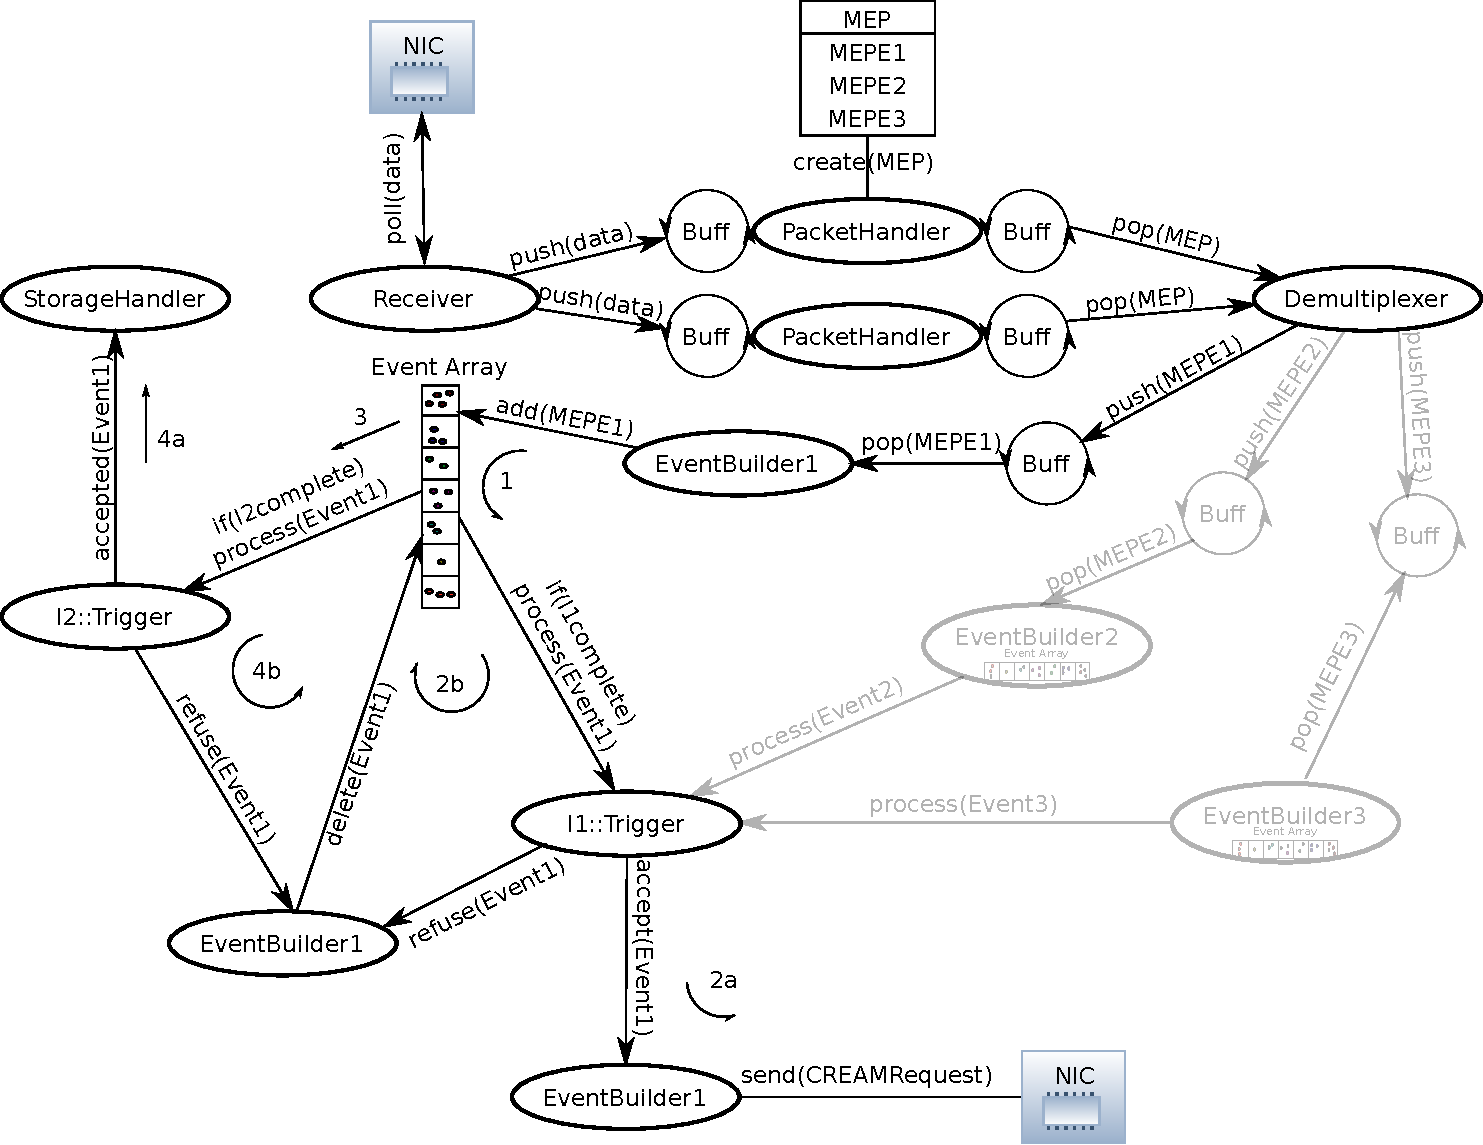
\includegraphics[width=9cm]{farm-concept}
	\end{center} 
\end{frame}

\begin{frame}{Circular buffers make the farm boy smile}{}
	\begin{center} 
		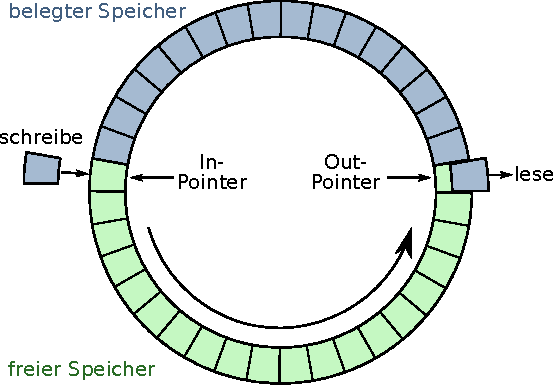
\includegraphics[width=8cm]{ringpuffer}
	\end{center} 
\end{frame}

\begin{frame}{Circular buffers for synchronization}{}
	\begin{center} 
		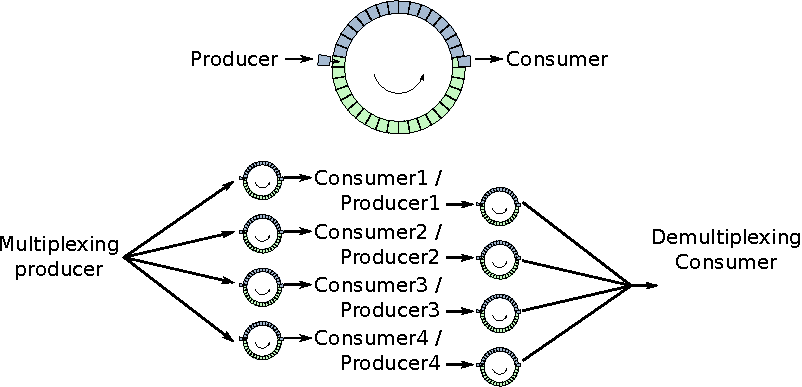
\includegraphics[width=8cm]{consumer-producer-queue}
	\end{center} 
\end{frame}

\begin{frame}[fragile]
\frametitle{Polling the buffer}
\begin{lstlisting}[frame=trBL,caption={}]{hallowelt}
while (true) {
  if (queue.pop(object)) {
    sleepMicros = 1; // slow start
    doSomething(object);
  } else {
    // The queue is empty! 
    usleep(sleepMicros);
    if (sleepMicros < 1E4) {
      sleepMicros *= 2;
    }
  }
}			
\end{lstlisting}
\end{frame}

\begin{frame}{Resulting CPU load}{}
	\begin{block}{Passive polling} 
		0.015\% CPU in Idle
	\end{block} 
	
		\begin{block}{Active polling every 10$\mus s$} 
		0.28\% CPU in Idle
	\end{block} 
\end{frame}